\section{Referenzen}

\subsection{ und Literaturverzeichnis}


\begin{frame}[fragile,t]
\frametitle{Bibliographien mit \texttt{thebibliography}}
\begin{itemize}[<+->]
  \item \textbf{Eine} einfache Möglichkeit in LaTeX eine Bibliographie zu erstellen.
  \item Dieses Vorgehen hat den Vorteil, dass im Gegensatz zu BibTeX \textbf{\texttt{<Inhalt der Referenz>}} den eingenen Ansprüchen entsprechend, einfach formatiert werden kann.
  \begin{enumerate}[<+->]
\item Einfügen der \texttt{thebibliography}-Umgebung vor \texttt{$\backslash$end\{document\}}
  \begin{center}
  \lstinline[style=Latex]+\begin{thebibliography}{99}+\\
  $\vdots$\\
   \lstinline[style=Latex]+\end{thebibliography}+
  \end{center}
  \item Erstellen von Einträgen innerhalb dieser Umgebung durch:
  \begin{center}
  \lstinline[style=Latex]+\bibitem{<Referenzname>} <Inhalt der Referenz>+
  \end{center}
  \item Aufrufen der Literaturangaben im Text durch
  \begin{center}
  \lstinline[style=Latex]+\cite{<Referenzname>}+ 
  \end{center}
  \end{enumerate}
\end{itemize} 
\end{frame}

\begin{frame}[fragile,t]
\frametitle{Beispiel mit einer Referenz}
\begin{lstlisting}[style=Latex]
\documentclass[12pt]{article}
\begin{document}
This thesis bases on the empirical work of Frumkes \cite{brain}.

\begin{thebibliography}{99}
\bibitem{brain} Lewis B. Frumkes. (2001). ``\textit{How to Raise Your I.Q. by Eating Gifted Children}.'' iUniverse.
\end{thebibliography}
\end{document}
\end{lstlisting}
\end{frame}

\begin{frame}[fragile]
\frametitle{Beispiel Literaturangabe}
\result{
\begin{figure}[htbp]
    \centering
        %trim=left botm right top
        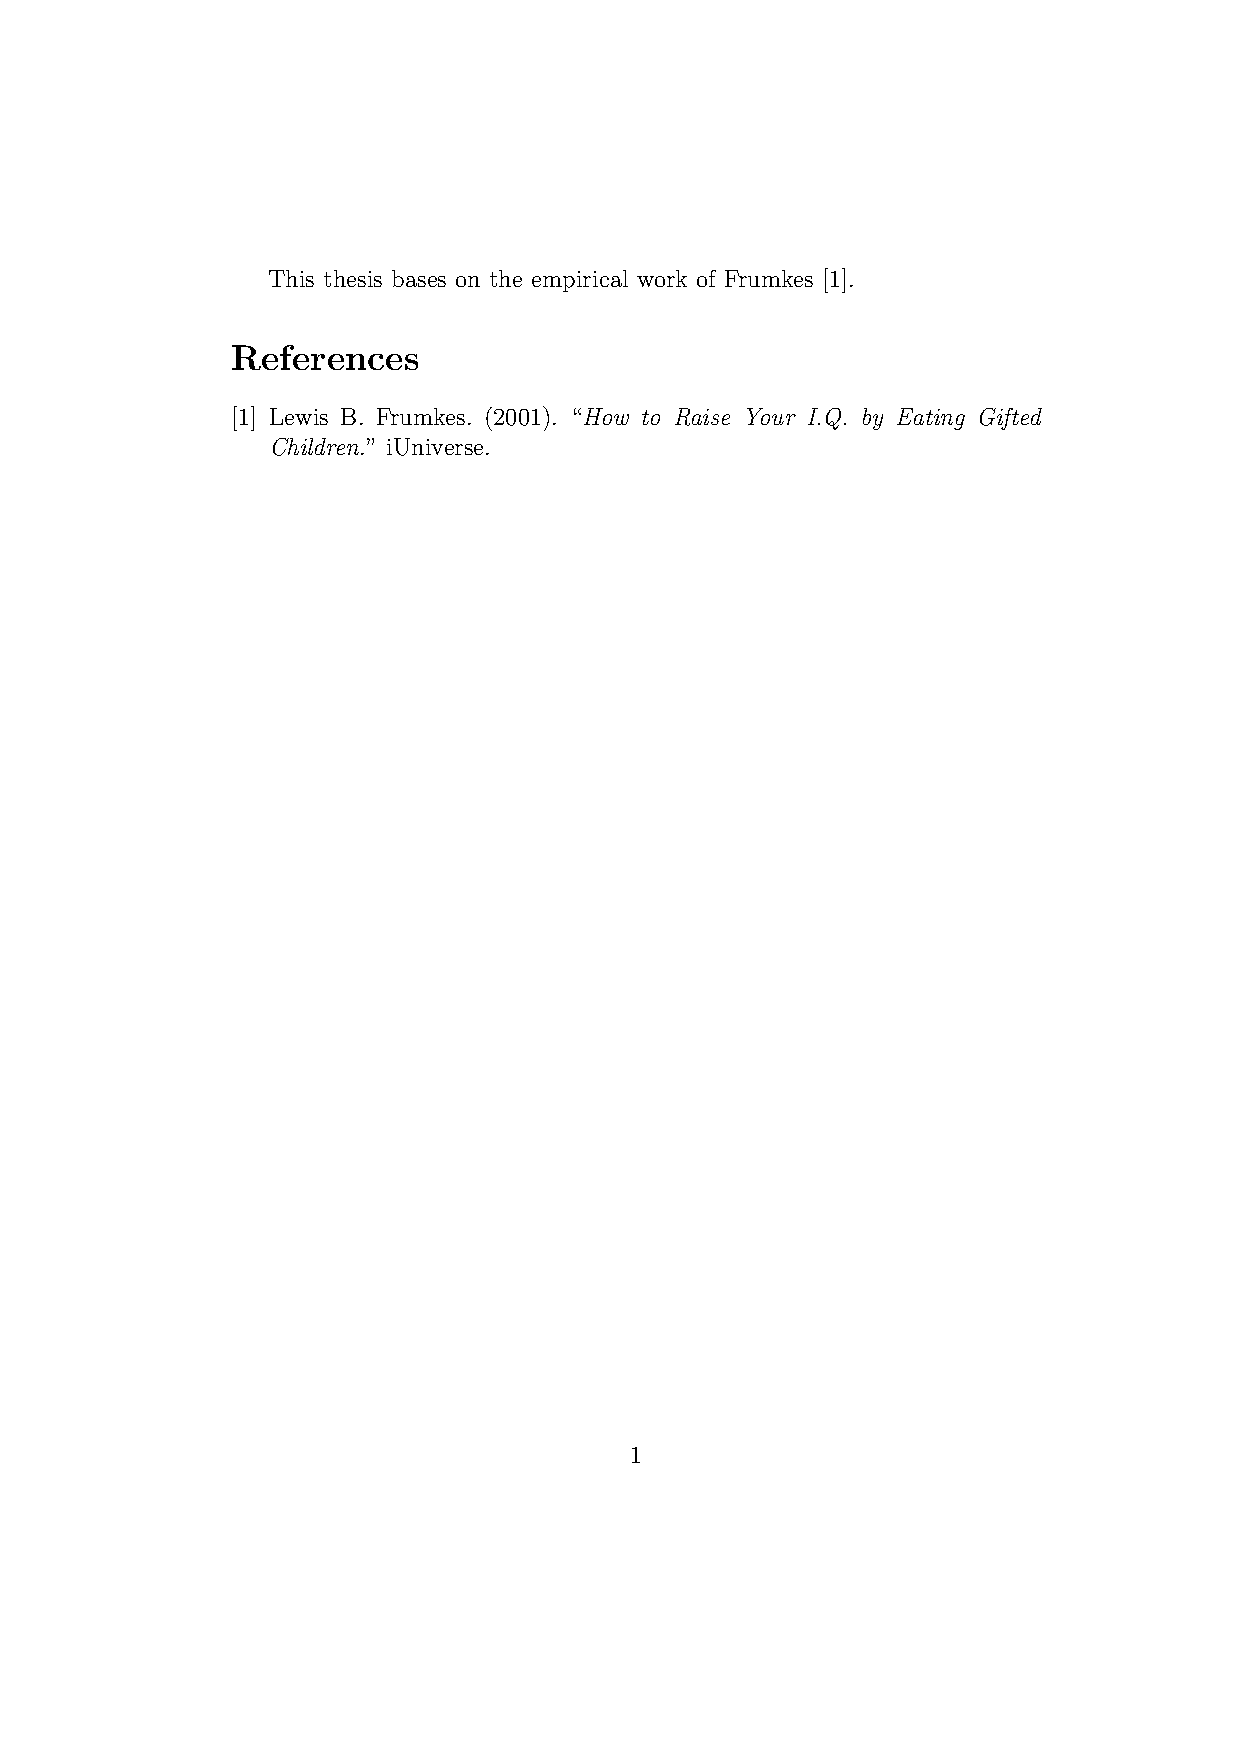
\includegraphics[clip, trim=3cm 22cm 0.5cm 4cm, width=1.00\textwidth]{images/Literaturangabe1.pdf}
    %\caption{Title}
    %\label{fig:somthing}
\end{figure}}
\end{frame}


\begin{frame}[fragile,t]
\frametitle{Beispiel mit mehreren Referenzen}
\begin{lstlisting}[style=Latex]
\documentclass[12pt]{article}
\begin{document}
This thesis bases on the empirical work of Frumkes \cite{brain}. The next theorem shows how to earn more money if you sell bulk trash. This work is founded by Dennis and Matthias \cite{money}.

\begin{thebibliography}{99}
\bibitem{brain} Lewis B. Frumkes. (2001). ``\textit{How to Raise Your I.Q. by Eating Gifted Children}.'' iUniverse.
\bibitem{money} Dennis K., Matthias D. (2017). ``\textit{How we earn more money}.'' Fachschaft VWL.
\end{thebibliography}
\end{document}
\end{lstlisting}
\end{frame}

\begin{frame}[fragile]
\frametitle{Beispiel Literaturangabe}
\result{
\begin{figure}[htbp]
    \centering
        %trim=left botm right top
        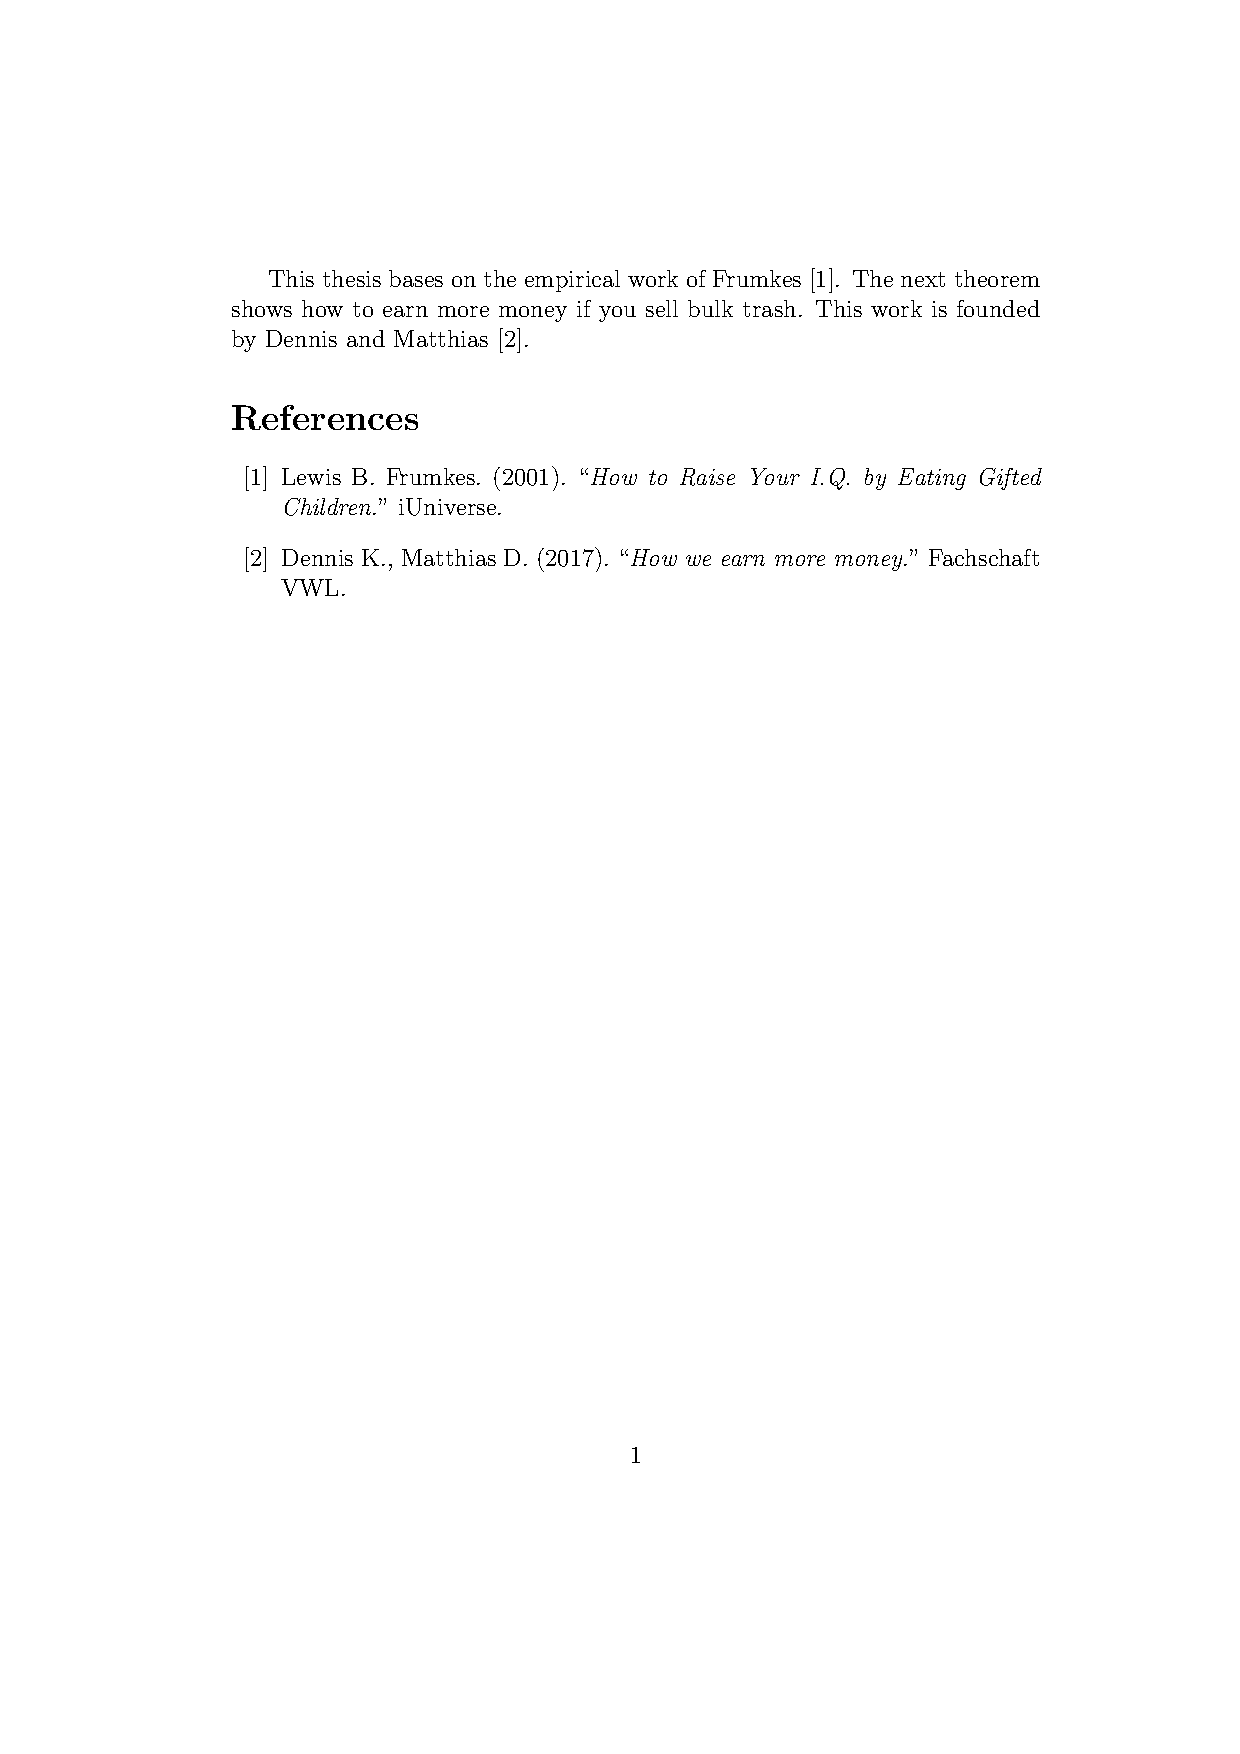
\includegraphics[clip, trim=3cm 19.5cm 0.5cm 4cm, width=1.00\textwidth]{images/Literaturangabe2.pdf}
    %\caption{Title}
    %\label{fig:somthing}
\end{figure}}
\end{frame}

\begin{frame}[fragile,t]
\frametitle{Andere Referenzstile}
Referenzieren mit Autor und Jahr in einer Klammer im Text \texttt{(<Autor>, Jahr)}:
\begin{itemize}[<+->] 
  \item In der Präambel müssen die folgenden Einträge vorgenommen werden:
   \begin{center}\lstinline[style=Latex]+\usepackage[authoryear]{natbib}+\end{center}
   \begin{center}\lstinline[style=Latex]+\setcitestyle{notesep={: }}+\end{center}
  \item In der Bibliographie muss jetzt der Inhalt der verweisenden Referenz angegeben werden: 
   \begin{center}\lstinline[style=Latex]+\bibitem[Autor/Autoren(Jahr)]{<Referenzname>} <Inhalt der Referenz>+\end{center}
   \item jetzt kann der Eintrag im eigentlichen Text referenziert werden: (\lstinline[style=Latex]+\citep+ muss verwendet werden)
    \begin{center}\lstinline[style=Latex]+\citep{<Referenzname>}+\end{center}
\end{itemize}
\end{frame}


\begin{frame}[fragile,t]
\frametitle{Beispiel andere Referenzstile}\vspace{-10pt}
\begin{lstlisting}[style=Latex]
\documentclass[12pt]{article}
\usepackage[authoryear]{natbib}
\setcitestyle{notesep={: }}

\begin{document}
This thesis bases on the empirical work of Frumkes \citep{brain}. The next theorem shows how to earn more money if you sell bulk trash. This work is founded by Dennis and Matthias \citep{money}.
\begin{thebibliography}{99}
\bibitem[Frumkes(2001)]{brain} Lewis B. Frumkes. (2001). ``\textit{How to Raise Your I.Q. by Eating Gifted Children}.'' iUniverse.
\bibitem[Dennis and Matthias(2017)]{money} Dennis K., Matthias D. (2017). ``\textit{How we earn more money}.'' Fachschaft VWL.
\end{thebibliography}
\end{document}
\end{lstlisting}
\end{frame}

\begin{frame}[fragile,t]
\frametitle{Beispiel andere Referenzstile}
\result{
\begin{figure}[htbp]
    \centering
        %trim=left botm right top
        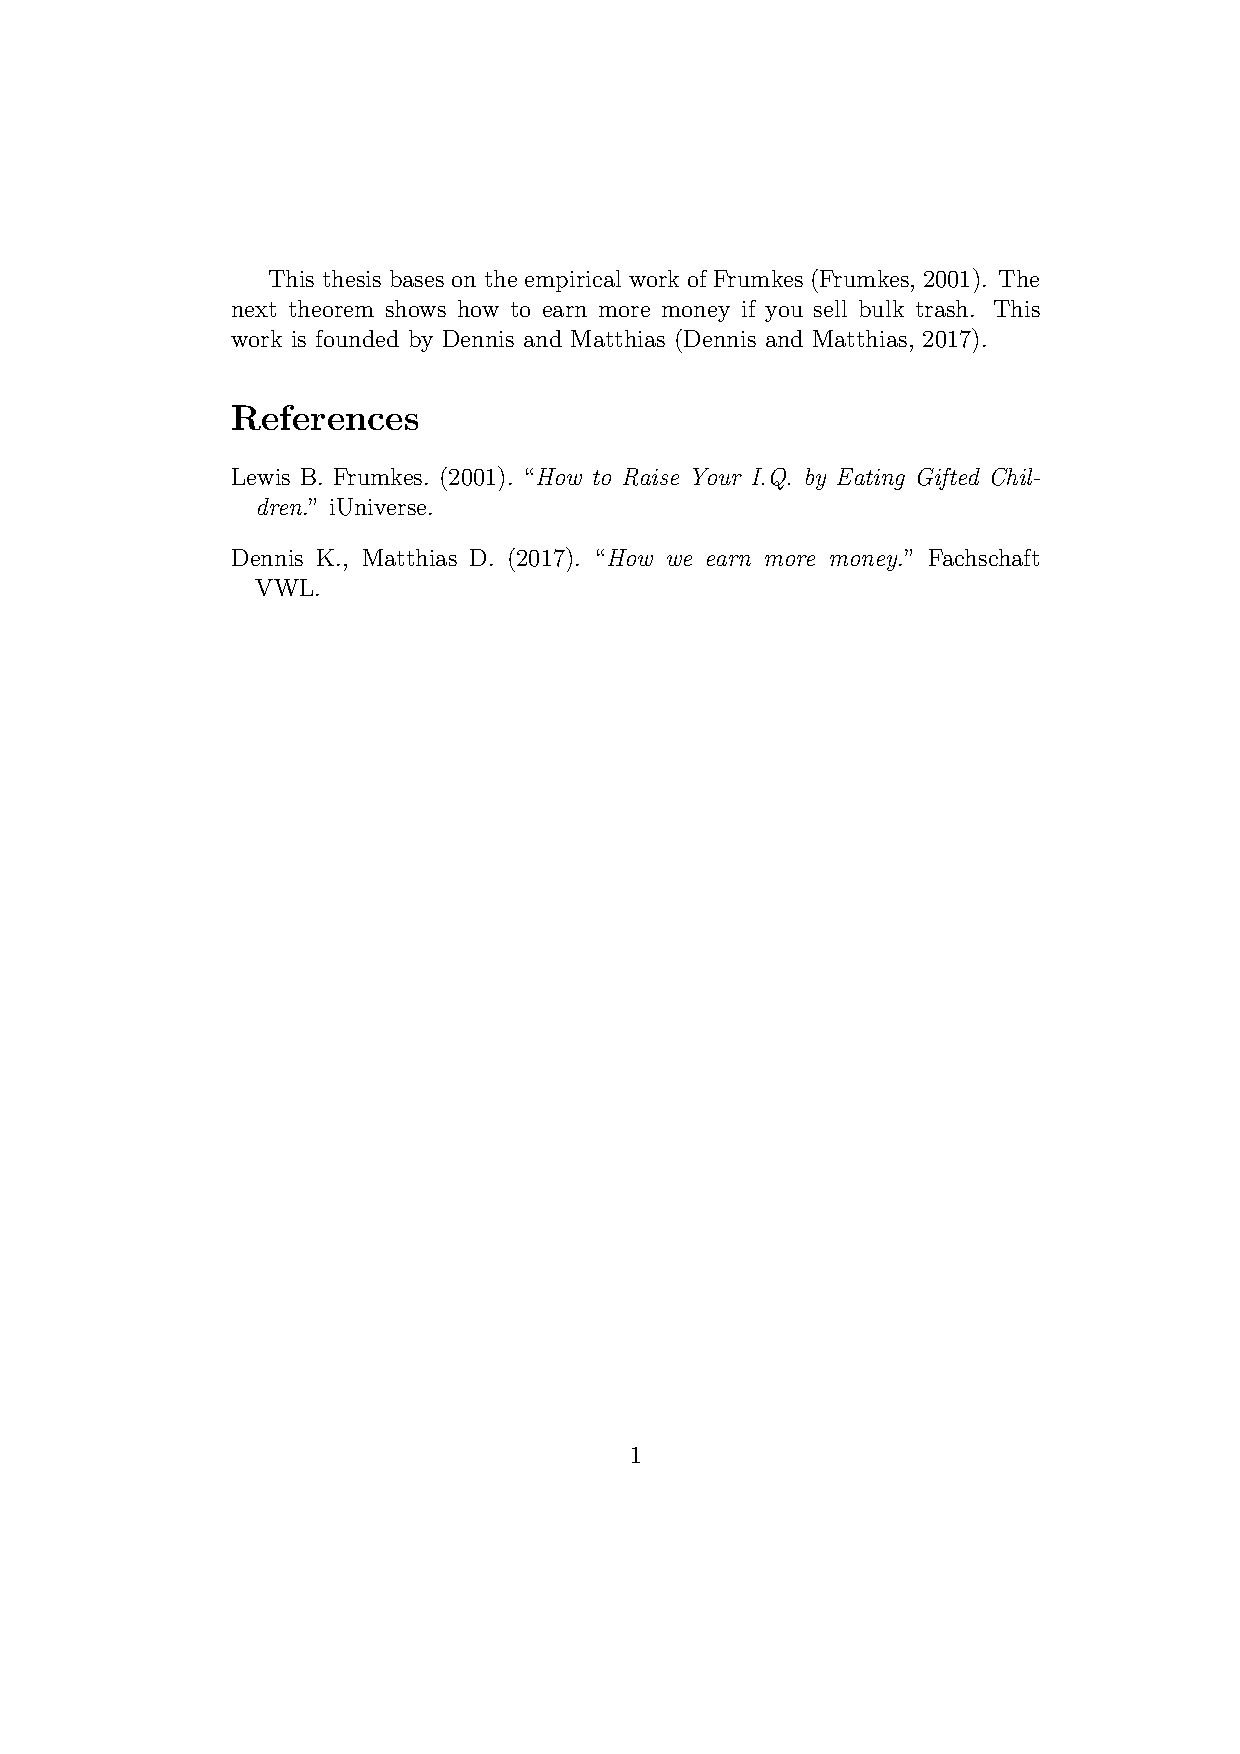
\includegraphics[clip, trim=3cm 19.5cm 0.5cm 4cm, width=1.00\textwidth]{images/Literaturangabe3.pdf}
    %\caption{Title}
    %\label{fig:somthing}
\end{figure}}
\end{frame}

\begin{frame}[fragile,t]
\frametitle{Zu beachten bei der Verwendung von \texttt{thebibliography}}
\begin{itemize}
\item Die Reihenfolge der \lstinline[style=Latex]+\bibitem+ Einträge legt die die Reihenfolge im LaTeX~Dokument fest
\item Die Bibliographieeinträge müssen alle von Hand formatiert werden
\item Bei Umfangreicheren Bibliographien sollte Biblatex verwendet werden. Dies führt jedoch auch zu mehr Aufwand. Wir verweisen hier auf entsprechende Seiten im Internet.
\end{itemize}
\end{frame}



\subsection{Referenzieren von Objekten}

\begin{frame}[fragile]
\frametitle{Referenzen}
\begin{itemize}[<+->]
  \item \LaTeX kann ''Verlinkungen'' zu table und figure-Umgebungen und Gleichungen erstellen
  \item Damit kann im Text auf die Nummerierung der Elemente zugegriffen werden
    \begin{itemize}[<+->]
      \item \lstinline[style=Latex]+\label{<Bezeichnung>}+ Dazu müssen die zu referenzierende Elemente mittels  ''verankert'' werden
      \item \lstinline[style=Latex]+\ref{<Bezeichnung>}+ Jetzt können diese durch abgefragt werden. 
      \item \lstinline[style=Latex]+\eqref{<Bezeichnung>}+ Handelt es sich um eine Gleichung, so kann  verwendet werden
    \end{itemize}
  \end{itemize}
\end{frame}


\begin{frame}[fragile]
\frametitle{Beispiel- ERSETZEM DURCH FIGURE ung gleichung}
\begin{lstlisting}[style=Latex]
\begin{satz}[genialer Satz]\label{satz:genial}
Dieser beinhaltet eine Formel:
\begin{equation}\label{eq:toll}
a^2 + b^2 = c^2
\end{equation}
\end{satz}
Satz \ref{satz:genial}, namentlich "`\nameref{satz:genial}"' 
auf Seite \pageref{satz:genial} beinhaltet die Formel \eqref{eq:toll}.
\end{lstlisting}
\pause
\end{frame}

\begin{frame}[fragile]
\frametitle{Beispiel}
\begin{satz}[genialer Satz]\label{satz:genial}
Dieser beinhaltet eine Formel:
\begin{equation}\label{eq:toll}
a^2 + b^2 = c^2
\end{equation}
\end{satz}
Satz \ref{satz:genial}, namentlich "`\nameref{satz:genial}"' 
auf Seite \pageref{satz:genial} beinhaltet die Formel \eqref{eq:toll}.
\end{frame}


\subsection{Fußnoten}

\begin{frame}[fragile]
\frametitle{Fußnoten}
\begin{itemize}[<+->]
  \item Fußnoten werden mittels \lstinline[style=Latex]+\footnote[<Nummer>]{<Text>}+ erzeugt.
  \item durch einen neuen \lstinline[style=Latex]+\chapter+ wird der Fußnotenzähler resettet.
  \item Es können auch andere Fußnotensymbole verwendet werden:
   \lstinline[style=Latex]+\renewcommand{\thefootnote}{\<ZiffStil>{footnote}}+ \\
   Dabei sind alle Ziffernstile, die auch für die Seitennummerierung gelten, sowie \texttt{fnysmbol} gültig.
\end{itemize}\pause
Beispiel:
\begin{lstlisting}[style=Latex]
Das ist ein toller Text\footnote{das die Notiz dazu}
\renewcommand{\thefootnote}{\fnysmbol{footnote}}
Das ist ein noch besserer Text\footnote{so sehen Symbole aus}
\renewcommand{\thefootnote}{\alph{footnote}}
Dies ist der letzte Text\footnote{mit Buchstaben}
\end{lstlisting}
Das ist ein toller Text\footnote{das die Notiz dazu}
\renewcommand{\thefootnote}{\fnsymbol{footnote}}
Das ist ein noch besserer Text\footnote{so sehen Symbole aus}
\renewcommand{\thefootnote}{\alph{footnote}}
Dies ist der letzte Text\footnote{mit Buchstaben}
\end{frame}

\begin{frame}[fragile]
\frametitle{Fußnoten}
\begin{itemize}[<+->]
  \item in manchen Fällen ist es Sinnvoll, Fußnote und Fußnotentext getrennt voneinander zu erstellen
  \item eine Fußnote kann manuell mit \lstinline[style=Latex]+\footnotemark[<Nummer>]+ erstellt werden
  \item wird keine Nummer angegeben, so wird der aktuelle Zähler um eins erhöht und als Fußnote verwendet. Die Angabe eine Nummer lässt den Zähler unberührt.
  \item über \lstinline[style=Latex]+\footnotetext[<Nummer>]{<Text>}+ kann ein Text erstellt werden. \texttt{<Nummer>} verhält sich hier genau wie oben.
  \item über diesen Weg lassen sich Fußnoten nahezu überall erstellen
\end{itemize}
\end{frame}

\begin{frame}[fragile]
\frametitle{Beispiel}
\begin{lstlisting}[style=latex]
Wir setzten eine Footnote \footnotemark[12] ...  
aber zeigen Sie auf einer anderen seite an.
\end{lstlisting}
Wir setzten eine Footnote \footnotemark[12] ...  
aber zeigen Sie auf einer anderen seite an
\end{frame}
\begin{frame}[fragile]
\begin{lstlisting}[style=latex]
\footnotetext[12]{hier}
\end{lstlisting}
\end{frame}
\footnotetext[12]{hier}

\subsection{Inhaltsverzeichnis}

\begin{frame}[fragile]
\frametitle{Inhaltsverzeichnis}
\begin{itemize}[<+->]
  \item mit dem Befehl \lstinline[style=Latex]+\tableofcontents+ wird eine \texttt{.toc}-Datei erstellt, in der alle Abschnitte aufgelistet werden
  \item beim erneuten compilieren wird diese Datei eingelesen und als Inhaltsverzeichnis ausgegeben
  \item<+-|alert@3> daher immer 2x compilieren! (3x bei langen Inhaltsverzeichnis)
  \item über den Befehl \lstinline[style=Latex]+\addtocontents{toc}{Eintrag}+ lässt sich manuell ein Eintrag in der \texttt{.toc}-Datei einfügen.\\
  \item über \lstinline[style=Latex]+\listoffigures+ oder \lstinline[style=Latex]+\listoftables+ lassen sich entsprechend analog Figuren- bzw. Tabellenverzeichnisse erstellen
  \item die Tiefe des Inhaltsverzeichnis wird über die Variable \texttt{tocdepth} gesteuert
\end{itemize}
\begin{lstlisting}[style=Latex]
\setcounter{tocdepth}{2}
\end{lstlisting}
\end{frame}

\subsection{Hyperref}

\begin{frame}[fragile]
\frametitle{Hyperref}
\begin{itemize}[<+->]
  \item das Paket \texttt{hyperref} sorgt dafür, dass Verlinkungen in \LaTeX\, anklickbare Hyperlinks erzeugen.
  \item dadurch werden die Befehle \lstinline[style=Latex]+\url{<URL>}+ bzw. \lstinline[style=Latex]+\href{<URL>}{<Text>}+ bereitgestellt, mit dem Internetadressen angegeben werden können
  \item außerdem wird der Befehl \lstinline[style=Latex]+\hypersetup+ definiert, mit dem Linkfarbe, PDF-Author und viele andere Dinge einstellbar sind. Weiteres dazu unter \url{http://en.wikibooks.org/wiki/LaTeX/Hyperlinks}
\end{itemize}
\end{frame}

\begin{frame}[fragile]
\textbf{Achtung:} Verwendet Ihr Hyperrefs in einem article Dokument, werden alle Links rot umrandet. Dies könnt unterbinden indem ihr Hyperref so einbindet:

\begin{lstlisting}[style=Latex]
\usepackage[colorlinks=false,pdfborder={0 0 0}]{hyperref}%Hide RED PDF Border
\end{lstlisting}

\end{frame}

